\PID \label{z:dtft_rec}
Нека је дат дискретан сигнал који представља правоугаони прозор полуширине $N$,  
$x[n] = \rect_N[n] = \begin{cases}
    1, |n| \leq N \\
    0, |n| > N
\end{cases}$. 
\begin{enumerate}[label=(\alph*)]
    \item Одредити и скицирати амплитудски спектар тога сигнала $|X(\jj\Omega)|$.
    \item Уколико се ширина главног лоба дефинише као растојање $\Delta \Omega$ између две нуле функције најближе 
    максимуму модула функције. Одредити ширину главног лоба. 
\end{enumerate}

\textsc{\underline{Решење}:}
Дискретна Фуријеова трансформација сигнала $x[n]$ се може одредити по дефиницији као 
$X(\jj\Omega) = \sum_{n = -\infty}^{\infty} x[n] z^{-n}$, где је $z = \ee^{\jj\Omega}$. Заменом датог облика сигнала 
у дефиницију има се\footnote{Користи се општији облик суме геометријске прогресије
    $\sum_{k = m}^n a q^k = a\dfrac{q^m - q^{n+1}}{1-q}$.
}
\begin{eqnarray}
    X[\jj\Omega] &=& \sum_{n = -\infty}^{\infty} \rect_N[n] z^{-n} = \sum_{n = -N}^N z^{-n} 
    = \dfrac{ z^{-(-N)} - z^{-(N+1)} }{1 - z} = 
    \dfrac{z^{N} - z^{-N-1}}{1 - z}. \label{eq:\ID.f1}
\end{eqnarray}
Да бисмо даље упростили дати резултат, потребно је да израз у бројицу изразимо у облику
\begin{eqnarray}
    z^a(z^b - z^{-b}) &=& z^{N} - z^{-N-1}  \\[2mm]
    z^{a+b} - z^{a-b} &=& z^{N} - z^{-N-1} \Rightarrow
    a+b = N\quad a-b = -N-1  
    \Rightarrow \\
    && a = \dfrac{1}{2}, \quad b = N + \dfrac{1}{2}.
\end{eqnarray}
На основу чега поједностављујемо израз \ref{eq:\ID.f1}, помоћу идентитета 
$z^n - z^{-n} = \jj 2 \sin(\Omega n)$, у облик 
\begin{equation}
    X(\jj\Omega) = \dfrac{ \cancel{z^{\frac12}}\left( z^{N + \frac12} - z^{-(N + \frac12)} \right)  }
    { \cancel{z^{\frac12}} \left( z^{\frac n2} - z^{-\frac n2} \right)}
    \Rightarrow
    X(\jj\Omega) 
    = \dfrac{\sin \left( \left(N + \frac12\right) \Omega \right) }{ \sin \left(  \frac12 \Omega \right)}
    \label{\ID:eq_rez}
\end{equation}

Добијена функција има облик познате \textit{Дирихлеове функције} и као таква се може наћи у софтверским  
алатима под називима \texttt{drcl} или \texttt{diric}. За неколико различитих вредности полуширине прозора, 
$N \in \{2,4,6\}$, на слици \ref{fig:\ID.varn} нацртани су амплитудски спектри на њиховом 
основном периоду. Максимална вредност амплитудског спектра постоји за $\Omega = 0$, када је на 
основу \eqref{\ID:eq_rez}, 
$\max |X(0)| = \lim_{\Omega \to 0}  \dfrac{\sin \left( \left(N + \frac12\right) \Omega \right) }{ \sin \left(  \frac12 \Omega \right)} 
= 2N + 1$, односно расте линеарно са ширином прозора.
\begin{figure}
    \centering
    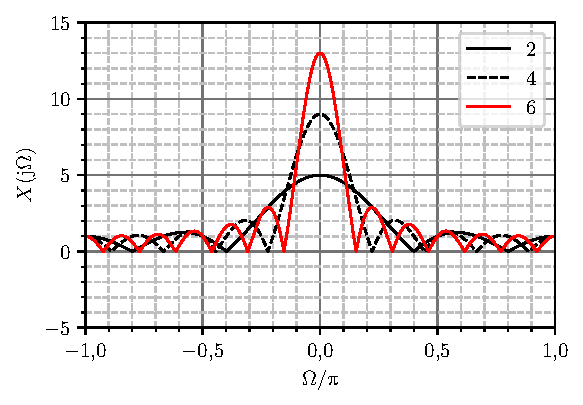
\includegraphics{fig/rec_spect_varn.pdf}
    \caption{Амплитудски спектар правоугаоног прозора за разне ширине $N$}
    \label{fig:\ID.varn}
\end{figure}

(б) Максимална вредност постоји за $\Omega = 0$, а границе главног лоба су на месту где су најближе 
нуле амплитудског спектра. То се дешава када је аругмент синусне функције у бројиоцу једнак $\pm \uppi$. 
На основу тога је 
\begin{equation}
    \left( N + \dfrac{1}{2} \right) \dfrac{\Delta \Omega}{2} = \uppi 
    \Rightarrow
    \Delta \Omega = \dfrac{2 \uppi}{N + \frac{1}{2}}.
\end{equation}
Дакле, као што се може видети на слици \ref{fig:\ID.varn} ширина главног лоба се сужава са повећањем ширине прозора. \\